% ChamberSim Reloaded - user manual.   Build: docs/manual/build.sh   (program version from CMakeLists.txt; raise \manualversion when the manual changes)
\documentclass[11pt,a4paper]{article}

\usepackage[utf8]{inputenc}
\usepackage[T1]{fontenc}
\usepackage{lmodern}
\usepackage[american]{babel}
\usepackage[margin=2.5cm]{geometry}
\usepackage{graphicx}
\usepackage{booktabs}
\usepackage{array}
\usepackage{xcolor}
\usepackage{tcolorbox}
\usepackage{enumitem}
\usepackage{fancyhdr}
\usepackage[hidelinks]{hyperref}

\graphicspath{{images/}}
\setlist{itemsep=2pt,topsep=4pt}
\setlength{\parindent}{0pt}
\setlength{\parskip}{6pt}

% Two versions: the manual's own revision, and the program version it describes (build.sh takes the latter from CMakeLists.txt)
\newcommand{\manualversion}{1.2}
\providecommand{\programversion}{0.3}

\definecolor{accent}{HTML}{2A7FBF}
\setlength{\headheight}{14pt}
\pagestyle{fancy}
\fancyhf{}
\fancyhead[L]{ChamberSim Reloaded -- User Manual}
\fancyhead[R]{\leftmark}
\fancyfoot[C]{\thepage}

% Menu paths and interface elements
\newcommand{\ui}[1]{\textsf{#1}}
\newcommand{\menu}[1]{\textsf{\textbf{#1}}}
\newcommand{\sep}{\,$\triangleright$\,}
\newcommand{\file}[1]{\texttt{#1}}

\newtcolorbox{warning}{colback=red!6,colframe=red!60!black,title=Safety,fonttitle=\bfseries,boxrule=0.6pt}
\newtcolorbox{note}{colback=accent!6,colframe=accent,title=Note,fonttitle=\bfseries,boxrule=0.6pt}

\title{
\includegraphics[width=3.5cm]{logo.png}\\[0.8cm]\Huge\textbf{ChamberSim Reloaded}\\[4pt]\Large Interior ballistics for handloaders\\[1.2cm]\huge User Manual}
\author{}
\date{Manual version \manualversion\\[2pt]for ChamberSim Reloaded version \programversion}

\begin{document}
\maketitle
\thispagestyle{empty}

\vfill
\begin{warning}
The results of this program are \emph{calculated}. They can differ considerably from reality.
Compare every load with the current loading tables of the component manufacturers and start low.
The software is provided ``as is'', without warranty of any kind. The author and all contributors accept no
responsibility or liability for any damage, injury or death or any other consequence of using this software or its results,
including damage to firearms or property. Reloading ammunition is dangerous and is done entirely at your own responsibility.
\end{warning}

\textit{ChamberSim Reloaded is an independent project. It is not affiliated with, endorsed or supported by Gordon's Reloading Tool
or its author.}

\newpage
\tableofcontents
\newpage

%=====================================================================
\section{Introduction}

ChamberSim Reloaded calculates the \emph{interior ballistics} of a handload: you choose a cartridge, a bullet and a powder, enter
the powder charge, and the program simulates how the pressure, the bullet velocity and the bullet energy develop while the
bullet travels through the barrel. From that it reports the maximum pressure, the muzzle velocity, the barrel time and many
related values. A load development ladder, charts, reports and printouts help to plan a series of test loads.

It follows the workflow of \emph{Gordon's Reloading Tool} (GRT). It can open the original's \file{.grtload} files and can use
the original's database, but stores its own loads in the \file{.csrload} format.

\subsection{What the program can do}
\begin{itemize}
  \item Cartridge, projectile and propellant records from a database; replace any component of a load; add your own records.
  \item Pressure, energy and velocity curves with markers and pressure bands, a burn-rate chart and a load ladder.
  \item Drawings of the cartridge and the chamber with the C.I.P.\ dimensions.
  \item A \ui{Measurements} tab for chronograph and pressure data, with statistics (mean, SD, ES) and a comparison with the simulation.
  \item \ui{Fit to measurements}: adapts the model values of a powder to your own data.
  \item Reports with a template editor, print preview and PDF export.
  \item Metric, imperial and original units (also per field), light and dark themes, adjustable font size.
  \item Translations: English, German, French and Italian.
\end{itemize}

\subsection{How accurate is it?}
The default \emph{Physical Model} is fitted to published load data of powder manufacturers. Against loads that were left out of the
fit, the muzzle velocity is typically within 3--6\,\% (root mean square; Vihtavuori powders about 3\,\%, Hodgdon about 6\,\%) and the peak pressure
within about 15\,\% where the tables publish it. The scatter of the published tables themselves (lots, barrels, components) is of that size.
Single loads can deviate much more. Unusual loads, other powders and other cartridges than the ones tested can deviate more again; slow powders
at low pressure, pistol and revolver cartridges (about 8\,\% in velocity and 19\,\% in pressure) and shotgun loads (about 3\,\% in velocity and 16\,\%
in pressure, with their own constants) are known weak spots. Powders without physical burn values, such as your own records, are less accurate than
the project's powders. The \ui{GRT Original} model reproduces the results of the original program to about 1\,\% in velocity and 3\,\% in pressure.
The files \file{README.md} and \file{docs/ACCURACY.md} of the project contain the current accuracy tables.

\begin{warning}
Never use a calculated load without checking it against the manufacturer's data. Work up from a safe starting charge and watch
for signs of excessive pressure.
\end{warning}

%=====================================================================
\section{Installation and first start}

\subsection{Installing}
Release builds are available from the project's GitHub page: an AppImage for Linux and a zip file for Windows. Unpack or
make the AppImage executable and start it; no installation is needed. Both contain this manual (\menu{Help}\sep\ui{User manual}, F1); the Windows zip also
contains the Visual C++ runtime, so nothing else has to be installed.
To build the program yourself you need Qt 6.4 or newer, CMake 3.16 or newer and a C++20 compiler:
\begin{verbatim}
tools/build.sh release
build/release/ChamberSimReloaded
\end{verbatim}

\subsection{Safety notice}
At every start a safety notice is shown. Read it, then choose \ui{I understand}; \ui{Quit} closes the program. With \ui{Do not show this again}
ticked, \ui{I understand} also switches the notice off for later starts. There is no entry in the settings to bring it back.

\subsection{Command-line options}
\begin{verbatim}
ChamberSimReloaded [options] [load.csrload ...]
  -d, --database <file> the original's (plain) database
  -r, --reference <f>   overlay a reference result (JSON) on the chart
  --calibration <m>     solver model: original|published|physical
  --language <code>     de_DE, en_US, fr_FR, it_IT
  --theme <t>           light | dark
  --units <system>      metric | imperial | original
  --log-level <level>   debug | info | warning | error
  --help                all options
\end{verbatim}
Files given on the command line are opened as loads. \texttt{-{}-theme} applies to this run only; \texttt{-{}-units} and \texttt{-{}-calibration}
are saved like the choices in the settings. \texttt{-{}-screenshot} saves an image of the window and exits (for documentation; see \texttt{-{}-help} for
\texttt{-{}-tab}, \texttt{-{}-input-tab} and \texttt{-{}-result-tab}).

\subsection{Simulating without the window}\label{sec:csrsim}
The program \texttt{csr\_sim} runs simulations without a graphical interface, for scripts and batch jobs. It reads \texttt{.csrload} and
\texttt{.grtload} files and prints one row per load and ladder step.
\begin{verbatim}
csr_sim [options] load.csrload|load.grtload ...
  --profile <m>         original | published | physical (default)
  --grt-original        use the Original model for .grtload files
  --charge <g>          override the charge of the load
  --ladder-count <n>    override the number of ladder steps
  --ladder-step <g>     override the charge difference of the ladder
  --format <f>          table (default) | csv | json
  --out <file>          write the results to a file
  --curve <file.csv>    pressure/velocity curve of the focused ladder step;
                        {name} is replaced by the load's file name
  --steps <n>           position steps of the solver (default 2000)
\end{verbatim}
The program's project data (physical burn values of the powders and the factors of the pistol and revolver calibers) are built in, so the results
equal those of the program. Each row holds the charge, maximum and muzzle pressure, muzzle velocity, energy and time, burnt fraction, efficiency, burnout in the barrel,
load ratio and the status. Units are g, mm, bar, m/s, J and ms, whatever the unit settings of the program. The exit code is 0 when all
simulations succeeded, 1 when at least one failed (for example because the charge does not fit into the case) and 2 for a usage or file error.

%=====================================================================
\section{The main window}

The window has a menu bar and, below it, a row of tabs. The first tab, \ui{Database}, is always present; every open load
gets a tab of its own. On Linux the program draws its own title bar with the menu in the title row
(\menu{File}\sep\ui{Settings}\sep\ui{Appearance}).

\begin{figure}[ht]
  \centering
  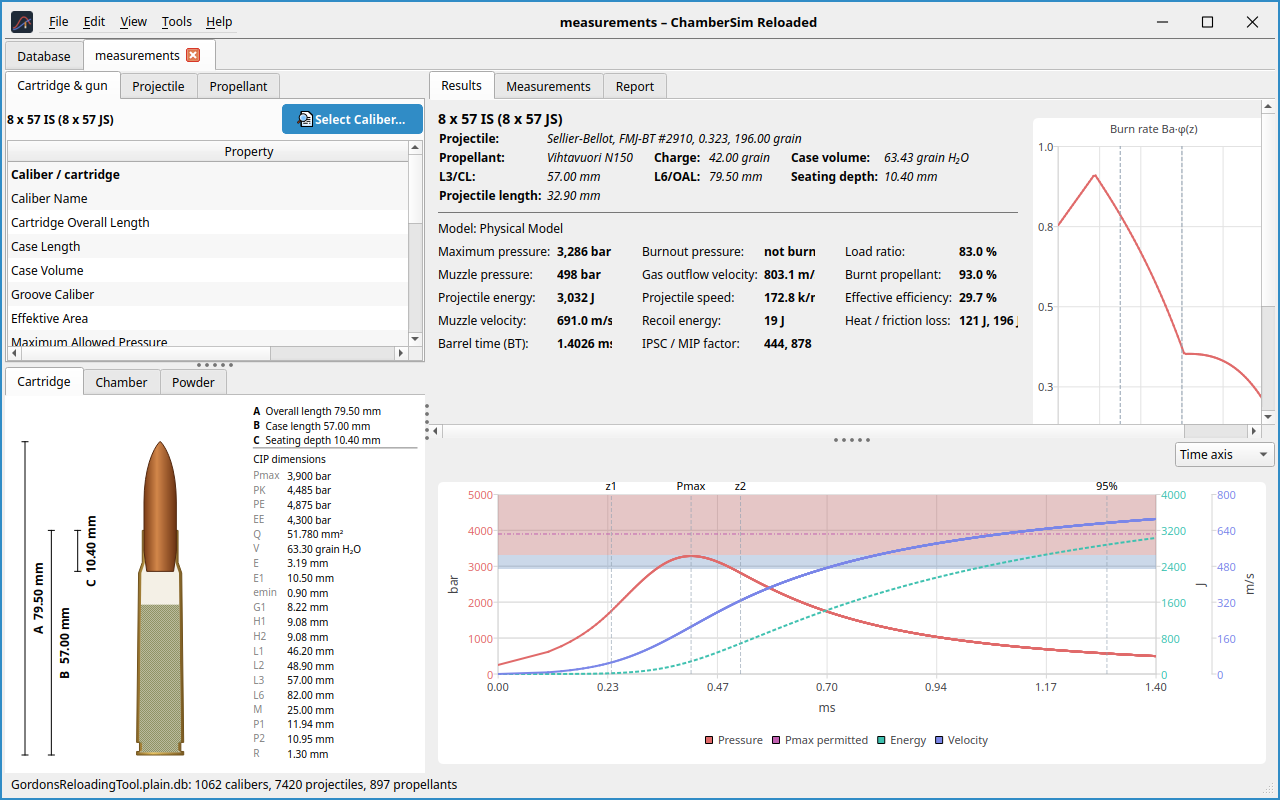
\includegraphics[width=\textwidth]{main.png}
  \caption{A load. Left: the input tabs (top) and the drawings (bottom). Right: results, measurements and report.}
  \label{fig:main}
\end{figure}

\subsection{Menus}
\begin{description}[style=nextline]
  \item[\menu{File}] \ui{New load\dots} (Ctrl+N), \ui{Open load\dots} (Ctrl+O), \ui{Open recent}, \ui{Save} (Ctrl+S),
    \ui{Save as\dots}, \ui{Print preview\dots}, \ui{Print\dots} (Ctrl+P), \ui{Export report as PDF\dots},
    \ui{Overlay reference result\dots} (Ctrl+R), \ui{Clear reference overlay}, \ui{Settings\dots} (Ctrl+,) and \ui{Quit}.
  \item[\menu{Edit}] \ui{Undo} (Ctrl+Z) and \ui{Redo} (Ctrl+Shift+Z or Ctrl+Y) for the load that is shown; see Section~\ref{sec:undo}.
  \item[\menu{View}] \ui{Theme} (system default, light, dark) and \ui{Language}. A language change takes effect after a restart.
  \item[\menu{Tools}] \ui{Burn rate table\dots} and \ui{Unit converter\dots}.
  \item[\menu{Help}] \ui{User manual} (F1), which opens this manual as a PDF, and \ui{About ChamberSim Reloaded\dots}
\end{description}

\subsection{Layout}
The panels are separated by splitters (the small dotted handles) that you can drag. The program remembers the splitter
positions, the column widths of the property tables and the window geometry.

%=====================================================================
\section{The database}\label{sec:db}

The \ui{Database} tab (Figure~\ref{fig:database}) lists the \ui{Calibers}, \ui{Projectiles} and \ui{Propellants} that are available
for loads. The filter field searches all columns; click a column header to sort.

\begin{figure}[ht]
  \centering
  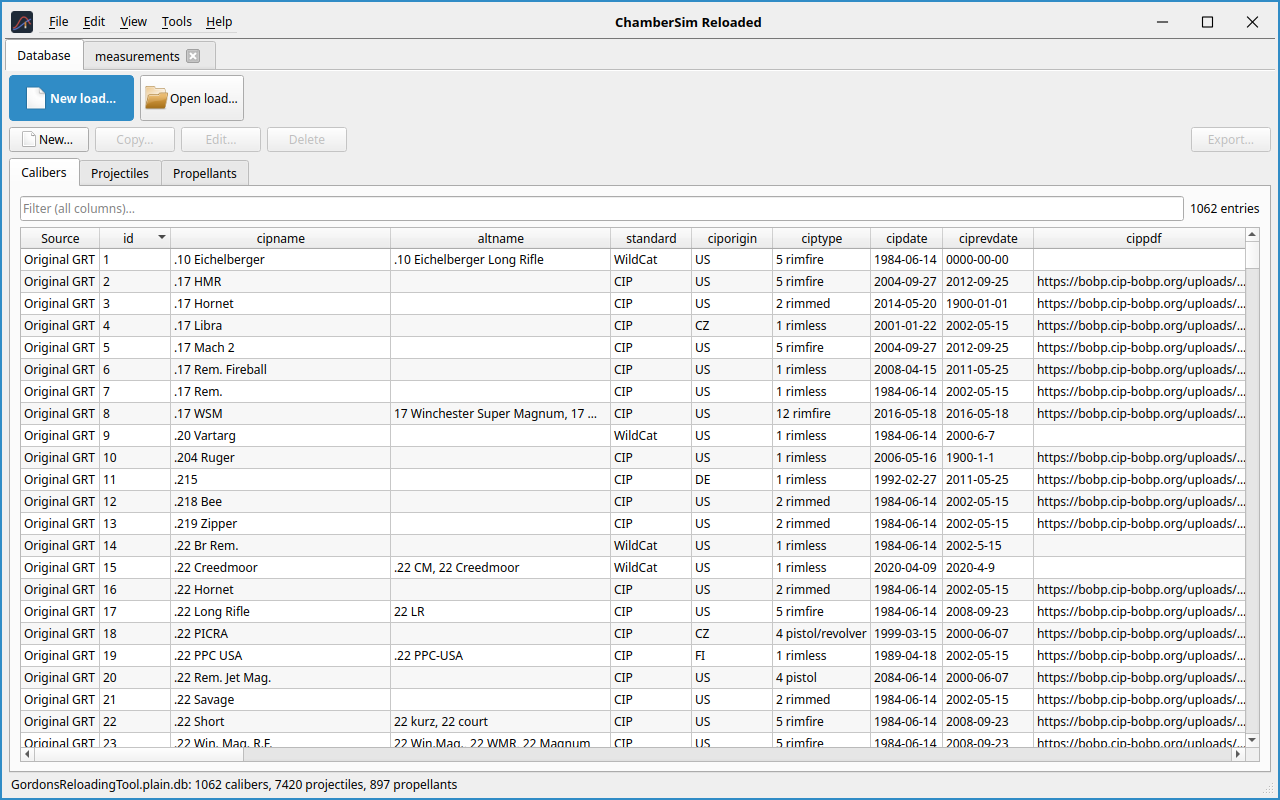
\includegraphics[width=\textwidth]{database.png}
  \caption{The Database tab.}
  \label{fig:database}
\end{figure}

\subsection{Where the records come from}\label{sec:sources}
The list is one view made of up to three sources, shown in the \ui{Source} column:
\begin{enumerate}
  \item The \textbf{project database}: calibers, projectiles and propellants that are built into the program.
  \item Your \textbf{own records}, stored in the file \file{ChamberSimReloaded.db} in the application data folder. Everything you create or copy
        is stored here.
  \item Optionally the records of \textbf{Gordon's Reloading Tool} (\ui{Original GRT}). The original's database is encrypted and must first be converted to a plain copy (Section~\ref{sec:dump}); choose that copy in \menu{File}\sep\ui{Settings}\sep\ui{Database}. It is only read, never changed.
\end{enumerate}

\subsection{Using the original's database}\label{sec:dump}
Gordon's Reloading Tool keeps its calibers, projectiles and propellants in an encrypted SQLite database (\file{GordonsReloadingTool.db}). ChamberSim Reloaded does not
decrypt it by itself and does not ship one. A helper script makes a \emph{plain} (unencrypted) \emph{copy} that you then choose in the settings. The program
and its database stay unchanged; only the copy is converted. You need your own installation of Gordon's Reloading Tool.

\paragraph{How it works.} The script starts a scratch copy of the original program. As soon as the original has unlocked its database, the script asks it to
remove the encryption from that copy. Nothing is compiled and no key is typed in.

\paragraph{Linux.}
\begin{enumerate}
  \item Unpack the \emph{Linux} version of Gordon's Reloading Tool. Its folder contains \file{GordonsReloadingTool}, \file{libs/} and \file{GordonsReloadingTool.db}.
  \item Copy \file{tools/grt\_decrypt\_db.sh} from the ChamberSim Reloaded sources into that folder.
  \item Open a terminal in that folder and run
\begin{verbatim}
./grt_decrypt_db.sh
\end{verbatim}
  \item The script checks what is needed and, after asking, installs what is missing with \texttt{sudo}: the debugger \texttt{gdb}, the 32-bit GTK~2 runtime that the
        original needs and, when no desktop is running, a virtual display. Debian/Ubuntu/Mint, Fedora, Arch/Manjaro and openSUSE are supported.
  \item After a few seconds the file \file{GordonsReloadingTool.plain.db} appears in the same folder.
\end{enumerate}
Options: \texttt{-o FILE} (name of the output file), \texttt{-y} (install without asking), \texttt{-c} (only report what is found and missing, change nothing),
\texttt{-{}-headless} (use a virtual display, no window appears), \texttt{-t SECONDS} (give up after this time, default 90) and \texttt{-h} (help).

\paragraph{Windows.}
\begin{enumerate}
  \item Copy \file{tools/grt\_decrypt\_db.cmd} and \file{tools/grt\_decrypt\_db.ps1} into the folder of Gordon's Reloading Tool (next to \file{GordonsReloadingTool.exe}).
  \item Double-click \file{grt\_decrypt\_db.cmd}. After asking, it installs Python (with \texttt{winget}) and the Python package \texttt{frida} into a private environment
        under \texttt{\%LOCALAPPDATA\%$\backslash$ChamberSimReloaded}.
  \item When it has finished, \file{GordonsReloadingTool.plain.db} is in the same folder.
\end{enumerate}
In PowerShell the options are \texttt{-Out FILE}, \texttt{-Yes}, \texttt{-Check} (report only) and \texttt{-Timeout SECONDS}.

\paragraph{Using the copy.} Open \menu{File}\sep\ui{Settings}\sep\ui{Database}, choose \file{GordonsReloadingTool.plain.db} as the \ui{Original database}.
The status line at the bottom then shows the file name and the number of calibers, projectiles and propellants, and the records appear in the \ui{Database} tab with
the source \ui{Original GRT}. They are read-only; to change one, make a copy. You can also start the program with \texttt{-d GordonsReloadingTool.plain.db}.

\begin{note}
Do not distribute the plain copy. It is for your own use with your own copy of Gordon's Reloading Tool. If the original program is updated, make a new copy.
\end{note}

\subsection{Working with records}
\begin{description}
  \item[New\dots] adds a new record. Fill in the fields; labels show the unit of each field.
  \item[Copy\dots] adds a changed copy of the selected record. A double click on a record shows it and offers the same.
  \item[Edit\dots] changes the selected record.
  \item[Delete] removes the selected record. Load files that use it keep their values.
  \item[Export\dots] saves the record as a file, to contribute it to the project's database.
\end{description}
Only your own records can be edited or deleted. To change a project or original record, make a copy.

For propellants you can attach an overview photo and a detail photo (\ui{Choose file\dots}, with the scale in px/mm if you know it).

%=====================================================================
\section{Making, opening and saving loads}\label{sec:files}

\subsection{New load}
\menu{File}\sep\ui{New load\dots} (Ctrl+N) opens a dialog with two steps.

\paragraph{Step 1: choose the components.} The tabs \ui{1.\ Caliber}, \ui{2.\ Projectile} and \ui{3.\ Propellant} list the records of the database. Select one record in each
tab; below the lists the dialog shows what you have chosen so far. The projectile list can be restricted to bullets that fit the caliber
(\ui{Show only bullets that fit the caliber}). \ui{Next >} becomes available when all three components are chosen.

\paragraph{Step 2: check the load data.} The dialog shows the chosen components and the \ui{Load data}: propellant charge, barrel length, bullet seating depth,
twist length and propellant temperature. They are filled with defaults for your selection (barrel length of the caliber, the cartridge at its maximum length, a charge of
70\,\% of the case capacity) and you can change them freely. The charge is also shown in the other mass unit (grams or grains).
\ui{Reset to defaults} restores the defaults.

\ui{< Back} returns to step 1. If you come back to step 2 with the \emph{same} three components, your changes are kept; if you change any component, the load data are filled in again
with the defaults of the new selection.

\ui{Create load} opens the new load in its own tab. It is called ``Untitled'' until you save it.

\subsection{Opening loads}
\menu{File}\sep\ui{Open load\dots} (Ctrl+O) opens one or several files at once; you can also give files on the command line. Each load gets its own tab,
named after the file. The file dialog offers three filters: all loads, \file{.csrload} only, and the original's \file{.grtload} only.
\begin{itemize}
  \item A load that is already open is not opened twice; its tab is shown instead.
  \item \menu{File}\sep\ui{Open recent} lists the last 12 loads. An entry whose file has disappeared or cannot be read is removed from the list.
  \item If a file cannot be read, a message names the file and the reason.
\end{itemize}

\subsection{Saving loads}
A tab with unsaved changes shows an asterisk after its name. \menu{File}\sep\ui{Save} (Ctrl+S) writes the load to its file; a new load (``Untitled'') and
\ui{Save as\dots} (Ctrl+Shift+S) ask for a file name. If you leave out the extension, \file{.csrload} is added.
When you close a tab or quit with unsaved changes the program asks whether to \ui{Save}, \ui{Discard} or \ui{Cancel}.

\subsection{The two file formats}
\begin{center}
\begin{tabular}{@{}lp{10cm}@{}}
  \toprule
  \file{.csrload} & The program's own format (XML). It contains everything: all input values, the caliber, projectile and propellant records
  with their values, the physical burn values of the Physical Model, the shotshell parts and your measurements and notes. \\
  \file{.grtload} & The format of Gordon's Reloading Tool. It can be opened and, as an export, written. \\
  \bottomrule
\end{tabular}
\end{center}
The format is chosen by the file name's extension.

\paragraph{Opening an original file.} A \file{.grtload} file is read completely, including the measurements, notes and pictures of its appendix. Because the program
saves only in its own format, \ui{Save} on such a load works like \ui{Save as\dots}: it suggests the same name with the extension \file{.csrload}. The original file
is never changed.

\paragraph{Exporting for the original program.} In \ui{Save as\dots} choose the filter \emph{Original GRT loads, without the data of ChamberSim Reloaded}
(or type a name ending in \file{.grtload}). The exported file can be opened in Gordon's Reloading Tool. It leaves out what that program does not know:
the physical burn values and the shotshell part choices. Keep a \file{.csrload} copy if you do not want to lose these.

\subsection{What a load file contains}
A load file is self-contained. The records of the caliber, projectile and propellant are stored in the file with their values, not as references to the
database. Consequently:
\begin{itemize}
  \item the load opens and calculates the same on another computer, without the original database;
  \item deleting or changing a record in the database does not change loads that were made with it (the program tells you so when you delete a record);
  \item to apply changes of a record to an existing load, select it again in the load (\ui{Select Propellant\dots} and so on); for a powder
        a banner points out that the load differs from the database, see section~\ref{sec:propellant}.
\end{itemize}
Measurement series, notes and pictures are part of the file as well. Parts of an original file that the program does not interpret are kept unchanged when you save.

\subsection{Undo and redo}\label{sec:undo}
Every load remembers its last 100 edits. \menu{Edit}\sep\ui{Undo} (Ctrl+Z) takes back the last edit and \menu{Edit}\sep\ui{Redo} (Ctrl+Shift+Z or Ctrl+Y) restores it again.
The menu entries name the edit, for example \ui{Undo Select Propellant}. The following edits are recorded:
\begin{itemize}
  \item changing a value in the property tables;
  \item choosing another caliber, projectile or propellant;
  \item applying the result of \ui{Fit to measurements} and accepting the physical burn values of a powder;
  \item changes in the \ui{Measurements} tab.
\end{itemize}
The history belongs to one load and is not saved in the file. It starts empty when a load is opened and is kept while the load is saved. If you undo back to the
state that was saved, the load no longer counts as modified. A new edit after an undo discards the steps that could have been redone.
Switching the selected ladder curve is not an edit that can be undone.

\subsection{Sessions}
The program remembers the loads that were open when you quit (only those that have a file). With \menu{File}\sep\ui{Settings}\sep\ui{Start-up}\sep
\ui{Open the loads of the last session at start} they are opened again at the next start, and the tab that was shown is selected again. Files that no longer
exist are skipped.

\subsection{Tips}
\begin{itemize}
  \item Save a load under a new name before you experiment with it; \ui{Save as\dots} leaves the old file as it is.
  \item Put the files of one rifle and component set into one folder and use the series of the \ui{Measurements} tab for the range sessions, so that a
        single file holds the history of a load.
  \item Files are plain XML text and suit version control or backup tools.
\end{itemize}

%=====================================================================
\section{Entering a load}

The left half of a load tab has three input tabs, the right half shows the results.

\subsection{Cartridge \& gun}
Shows the caliber (\ui{Select Caliber\dots} replaces it) and a table of properties: designation, overall length, case length, case volume,
bore, effective area, maximum permitted pressure, barrel length, twist length, seating depth and more. Below the table the
drawings show the cartridge, the chamber and (when available) the powder.

\paragraph{Replacing the caliber.} After you choose another caliber, the program can also set barrel length, seating depth and charge to the defaults
of the new caliber (tick the corresponding option in the selection dialog).

\subsection{Projectile}
Mass, diameter, length and the other bullet data. \ui{Select Projectile\dots} replaces the bullet; tick \ui{Show only bullets that fit the caliber}
to narrow the list. The \ui{Initial Gas Pressure} is the pressure at which the bullet starts to move and engraves. The \ui{Bullet friction} is an extra
resistance in bar that acts all along the barrel; it is always applied. Negative values are possible and describe low-friction bullets (the original's
database has values down to $-100$\,bar). For 362 rifle bullets the project records carry start pressure and friction values fitted to published loads.
A load keeps the values it was made with until you select the bullet again.

\subsection{Propellant}\label{sec:propellant}
Powder charge, explosion heat, burn rate and the form-function values. \ui{Select Propellant\dots} replaces the powder.

With the Physical Model, project powders also have \emph{physical burn values}. They are kept in the load file. If they are missing, an
orange banner tells you so and offers \ui{Use the physical values\dots}.

A load keeps its own copy of the powder values. If a database record of that powder was corrected after the load was made, or you edited the
values in the load, a second orange banner says \emph{Powder values differ from the database}. The load is still calculated with its own
values. \ui{Use the database values\dots} replaces them with those of the closest record (the charge and all other settings stay; \ui{Undo}
takes it back). A powder can have several records, so the banner appears only if no record has exactly the values of the load. With the
Physical Model only the project's records are compared, because the original database is not updated; with the other models all records count.

\subsection{Editing values}
Click a value in a property table to edit it. Values with a unit have a drop-down menu for the unit; the choice applies to this field only.
\ui{Reset per-field units} in the settings returns every field to the chosen unit system. Some fields are coded values (for example the
\ui{Shotshell} flag) and offer a list of choices.

\subsection{Measuring a load}
A good \ui{Case Volume} is the single most important input after the powder. Measure a fired case by filling it with water and weighing it.
Also measure the real bullet length and cartridge overall length and enter the mean values.

\subsection{Shotgun loads}
Calibers with \ui{Shotshell} set to yes use their own model terms. Enter such a load as follows:
\begin{itemize}
  \item \ui{Projectile}: mass = shot + wad (about 2.5\,g for a plastic wad), length = height of the shot column plus the wad,
        diameter = bore diameter;
  \item seated completely inside the hull: cartridge overall length = hull length, seating depth = projectile length;
  \item \ui{Initial Gas Pressure} = crimp release, about 20\,bar.
\end{itemize}
The load also has the choices \ui{Shotshell Hull}, \ui{Shotshell Wad} and \ui{Shotshell Primer}, each with three groups of similar parts
(low, medium and high pressure). They change the pressure by up to about $\pm 20\,\%$. Shotgun results are less reliable than rifle
and handgun results.

%=====================================================================
\section{Results}

\subsection{Results tab}
The \ui{Results} tab shows a summary of the load and the key values: maximum pressure, muzzle pressure, projectile energy, muzzle
velocity, barrel time, burnout pressure, gas outflow velocity, projectile speed (revolutions per minute), recoil energy, load ratio, the fraction of burnt
powder, the effective efficiency and the heat and friction loss. The model in use is named above the values.

Warnings appear in colored banners: \emph{Above the permitted maximum pressure}, \emph{Charge too high} (the charge does not fit into the case behind
the bullet) and \emph{Invalid input} (the simulation cannot run with these values). Two orange notices concern the powder: \emph{No physical burn
values} and \emph{Powder values differ from the database} (see section~\ref{sec:propellant}).

\subsection{Chart}
The big chart shows pressure, energy and velocity as curves. A drop-down menu switches the horizontal axis between time and position. Vertical
lines mark the transitions of the powder burn (z1, z2), the position of the maximum pressure, burnout and 95\,\% of the muzzle velocity. The colored
bands show the permitted maximum pressure. Move the mouse over the chart to read the values at that point.

\subsection{Burn-rate chart}
The smaller chart shows the burn rate $B_a\cdot\varphi(z)$ over the burnt fraction.

\subsection{Reference overlay}
\menu{File}\sep\ui{Overlay reference result\dots} (Ctrl+R) draws a saved result (a JSON file, for example from a run of the original program) as dashed
curves over the chart of the shown load, for comparison. \ui{Clear reference overlay} removes it.

\subsection{Load development ladder}
With a ladder, the program simulates several charges at once. Set the number of steps and the charge difference in the load's ladder fields; up to
ten steps are possible. The selected charge is the maximum, the further steps go down from there. A table (charge, maximum pressure, velocity, energy
and load ratio) and a row of tabs above the chart show the steps; click one to display its curve.

\subsection{Choosing the solver model}\label{sec:solver}
In \menu{File}\sep\ui{Settings}\sep\ui{Solver} you select the model:
\begin{description}
  \item[Physical Model] (default) A time-integrated model with flame spread, engraving, friction, air, heat loss and spin. It is fitted to published
        load data of the powder manufacturers.
  \item[Published] The GRT equations with empirical constants.
  \item[GRT Original] Calibrated against reference runs of the original program.
\end{description}
The model in use is shown in the results. The three models give different numbers; they are not exchangeable.

\paragraph{Original GRT files.} With \ui{Always use GRT Original for original GRT files (*.grtload)} a load whose file is a \file{.grtload} is
always calculated with GRT Original and the burn values in the file, whatever model is selected. Its results are then close to those Gordon's
Reloading Tool shows for the same file (the results line says \ui{GRT Original (original GRT file, \dots)}). Once the load is saved as a
\file{.csrload}, it uses the selected model again.

\begin{figure}[ht]
  \centering
  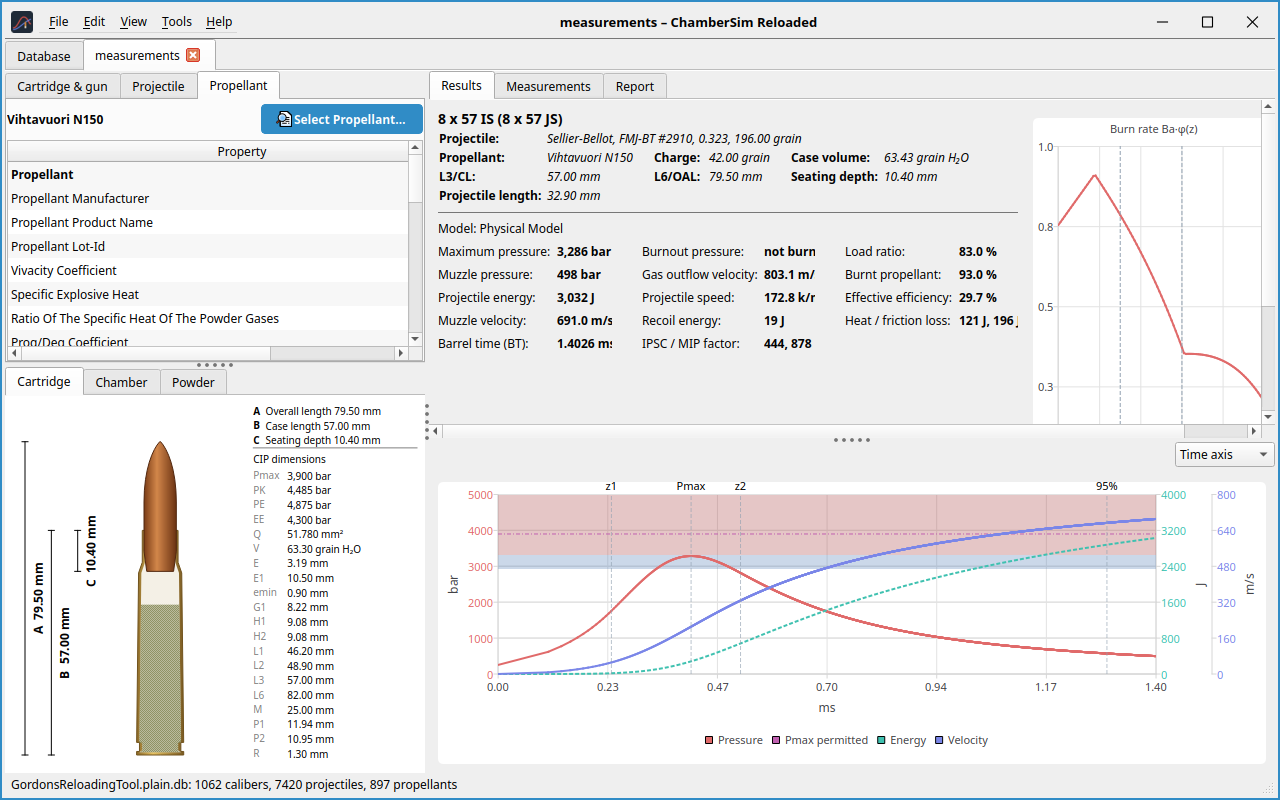
\includegraphics[width=\textwidth]{propellant.png}
  \caption{The Propellant input tab with results and chart.}
\end{figure}

%=====================================================================
\section{Measurements}

The \ui{Measurements} tab holds your own chronograph and pressure data. It is stored in the load file and used to compare the real load with the simulation
and to fit the powder model.

\begin{figure}[ht]
  \centering
  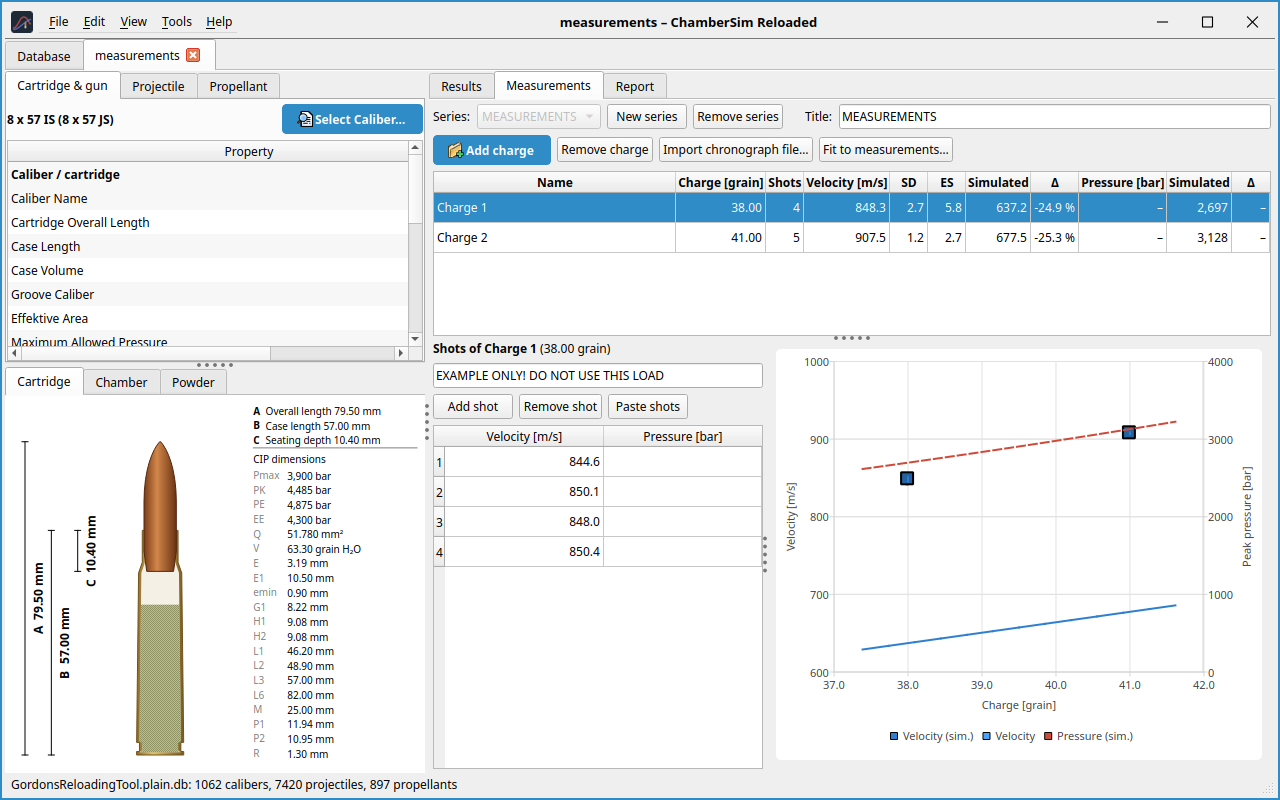
\includegraphics[width=\textwidth]{measurements.png}
  \caption{The Measurements tab.}
  \label{fig:meas}
\end{figure}

\subsection{Series and charges}
A load can have several \emph{series} (for example one per range day or rifle). \ui{New series} starts an empty series, \ui{Remove series} deletes the shown
one, and the title field names it. Inside a series:
\begin{description}
  \item[Add charge] adds a charge (the load's charge, or the next ladder charge). \ui{Add ladder charges} adds every ladder charge that is not listed yet.
  \item[Remove charge] removes the selected charge with all its shots.
\end{description}
The table has one row per charge: name, charge, number of shots, mean velocity, SD, ES, the simulated velocity and the difference ($\Delta$), then the same for the peak pressure.

\subsection{Shots}
Select a charge and enter the velocity (and pressure, if measured) of each shot. \ui{Add shot}, \ui{Remove shot} (Del) and \ui{Paste shots}
(one shot per line, velocity and optionally pressure) help. A note field per charge holds rifle, chronograph and conditions.

\subsection{Importing chronograph files}
\ui{Import chronograph file\dots} reads \textbf{Garmin Xero} files (the \file{.fit} file of the C1 Pro, or the CSV exported by the Garmin Xero app, in any language of the app), \textbf{MagnetoSpeed} CSV files
and \textbf{Labradar} \file{Report.csv} files. Missed shots (speed 0) are left out. These files do not contain the powder charge;
type it for each series in the import dialog.

\subsection{Statistics and chart}
The program computes the mean, the standard deviation (SD) and the extreme spread (ES, fastest minus slowest) of the velocity. The chart shows the
measured values and the simulated curve over the charge; hover the lines to read values.

\subsection{Fit to measurements}
\ui{Fit to measurements\dots} changes the propellant's model values until the simulation agrees with your data.

\begin{warning}
The result is only as good as your measurements and the powder data. Use it for planning, not as a replacement for the manufacturer's data.
\end{warning}

\begin{enumerate}
  \item \textbf{Prepare the load.} Enter a measured case volume and the real bullet and cartridge lengths.
  \item \textbf{Enter measurements.} The more different charges, the better: at least 5 shots per charge, 2 or more charges, ideally also 2 or more bullet weights or calibers.
  \item \textbf{Open the dialog} and choose the \emph{values to fit}. The default depends on the data: $B_a$ alone for fewer than 3 charges,
        $B_a$ and $a_0$ for 3 to 5, all four ($B_a$, $a_0$, $z_1$, $z_2$) for 6 or more charges from at least two load files.
  \item Click \ui{Fit}. The dialog lists velocity and pressure of every charge before and after the fit and the rms error. Read the warnings
        (for example: the case volume is only the database value, or there are fewer charges than values).
  \item Check the result: after the fit, velocity differences should be small (below about 2\,\%).
  \item \ui{Apply to this load} puts the values into this load only. \ui{Save as own propellant\dots} stores a new record ``\textit{name} (fitted)''
        in your own database, which you can then select in any load. With the Physical Model and a project powder, the fit changes the load's physical burn
        values instead and keeps them in the load.
\end{enumerate}

%=====================================================================
\section{Reports and printing}

The \ui{Report} tab shows a formatted report of the load (Figure~\ref{fig:report}). With \menu{File}\sep\ui{Print preview\dots}, \ui{Print\dots} and
\ui{Export report as PDF\dots} you output it. The report scale is adjustable.

\begin{figure}[ht]
  \centering
  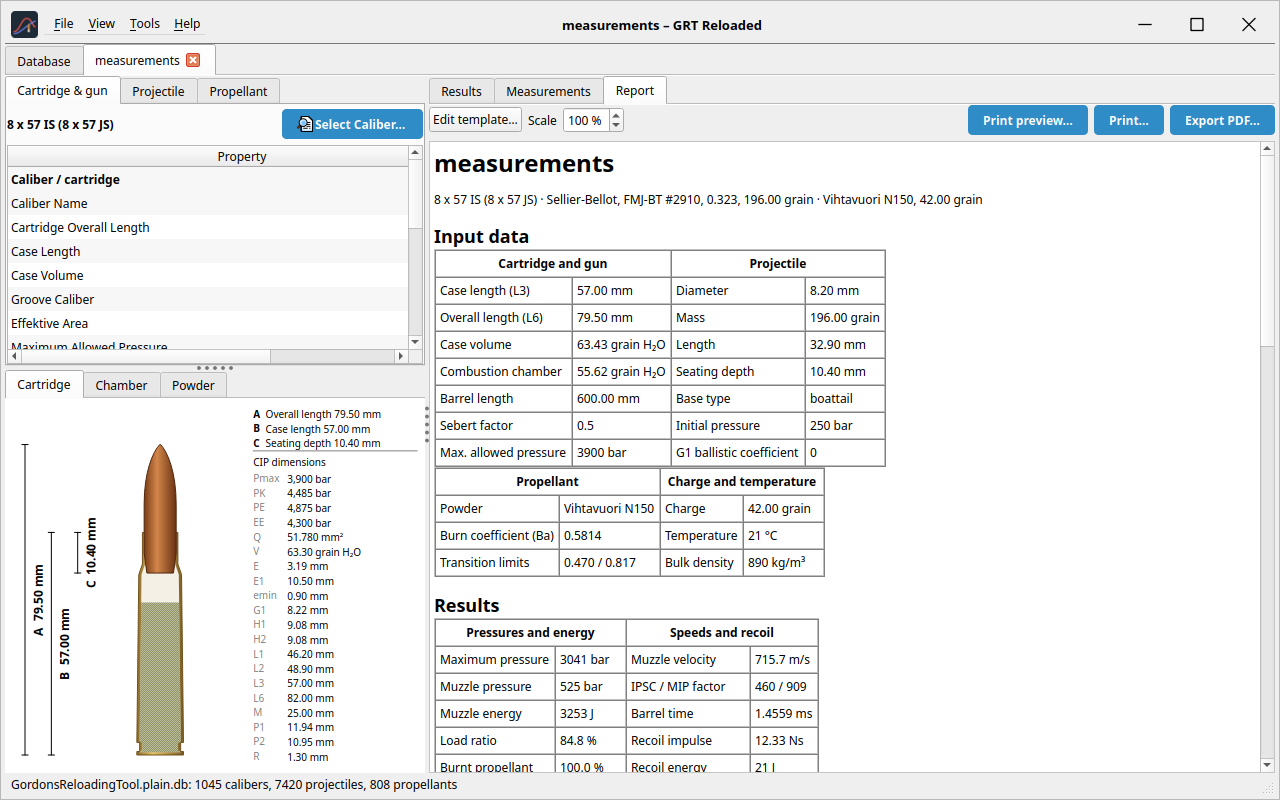
\includegraphics[width=\textwidth]{report.png}
  \caption{The Report tab.}
  \label{fig:report}
\end{figure}

\subsection{Report templates}
In the settings, \ui{Report template\dots} opens the template editor. A template is text with placeholders of the form
\texttt{\textasciitilde\textasciitilde source.property\textasciitilde\textasciitilde} or
\texttt{\textasciitilde\textasciitilde source.property("\#.00")\textasciitilde\textasciitilde} (with a number format). Use \ui{Insert value} to pick a placeholder
and \ui{Reset to default} to restore the standard template. The report of the Measurements tab includes only the selected series.

%=====================================================================
\section{Tools}

\subsection{Burn rate table}
\menu{Tools}\sep\ui{Burn rate table\dots} compares propellants by burn rate, brisance ($B_r$), progressivity ($B_p$) and the combined value ($B_{rp}$).
These factors are derived from the powder's $B_a$, explosion heat, $k$ and the form-function values; the solver does not use them.

\subsection{Unit converter}
\menu{Tools}\sep\ui{Unit converter\dots} converts between the units of the common quantities, for example grains and grams or bar and psi.

%=====================================================================
\section{Settings}

\menu{File}\sep\ui{Settings\dots} (Ctrl+,) has these groups:
\begin{description}
  \item[Database] The location of the original's \emph{plain} database (see Section~\ref{sec:dump}).
  \item[Units] The unit system (Metric, Imperial or Original) and \ui{Reset per-field units}.
  \item[Solver] The calculation model, and GRT Original for original GRT files (Section~\ref{sec:solver}).
  \item[Appearance] The \ui{Font size} (with a button for the system default), \ui{Custom Title Bar} (Linux: the program's own title bar with the menu
        in the title row) and \ui{Rounded Dialog Corners} (dialogs have their own frame with the custom title bar; this needs a compositing window
        manager and applies to dialogs opened afterwards). The theme is chosen in \menu{View}\sep\ui{Theme}, not here.
  \item[Start-up] \ui{Open the loads of the last session at start}. Not used when load files are given on the command line.
  \item[Logging] The log level (Debug, Info, Warning, Error or Off), output to the console and/or a log file, with \ui{Open log file} and \ui{Clear log file}.
\end{description}
\ui{Apply} puts the changes into effect and keeps the dialog open, \ui{OK} applies and closes it, and \ui{Cancel} also takes back what \ui{Apply} did.

%=====================================================================
\section{Tips and troubleshooting}

\begin{description}
  \item[``No original database'' in the status line.] No plain copy of the original's database has been chosen. The project's records still work. Choose one in
        \menu{File}\sep\ui{Settings}\sep\ui{Database} if you want the original's records.
  \item[Encrypted database error.] You chose the encrypted \file{GordonsReloadingTool.db}. Use the decrypted copy
        (see Section~\ref{sec:dump}).
  \item[``Charge too high''.] The charge does not fit into the case behind the bullet. Reduce the charge or increase the seating depth.
  \item[A record cannot be edited.] Only your own records can be changed. Make a copy first.
  \item[The pressure is much higher than in the loading manual.] Check the case volume, the powder lot, the seating depth and the bullet data. Try another
        model and compare. Always trust the manual over the calculation.
  \item[The language does not change.] The language change takes effect after a restart.
  \item[Something else.] Set the log level to \ui{Debug} and look at the log file.
\end{description}

\section{Glossary}
\begin{tabular}{@{}>{\raggedright\arraybackslash}p{3.2cm}p{11.5cm}@{}}
  \toprule
  Term & Meaning \\
  \midrule
  $B_a$ & Burn rate (vivacity) of the powder \\
  $a_0, z_1, z_2$ & Form-function values: the shape of the powder grain and the transitions of its burning \\
  $Q_{ex}$ & Explosion heat (energy content) of the powder \\
  $k$ & Ratio of the specific heats of the powder gases \\
  BT & Barrel time: time for the bullet to reach the muzzle \\
  SD / ES & Standard deviation and extreme spread of the velocity \\
  Load ratio & Fraction of the case that the powder fills (loading density) \\
  C.I.P. & Commission Internationale Permanente, which standardizes cartridge and chamber dimensions \\
  $P_{max}$ & Maximum permitted pressure \\
  \bottomrule
\end{tabular}

\end{document}
